\appendix
\chapter{Appendices}
\label{ch:appendices}

{}

Appendix 1

\includegraphics{figures/media/image27.emf}

Appendix 2

\begin{longtable}[]{@{}
  >{\raggedright\arraybackslash}p{(\columnwidth - 8\tabcolsep) * \real{0.1827}}
  >{\raggedright\arraybackslash}p{(\columnwidth - 8\tabcolsep) * \real{0.1243}}
  >{\raggedright\arraybackslash}p{(\columnwidth - 8\tabcolsep) * \real{0.2607}}
  >{\raggedright\arraybackslash}p{(\columnwidth - 8\tabcolsep) * \real{0.2343}}
  >{\raggedright\arraybackslash}p{(\columnwidth - 8\tabcolsep) * \real{0.1981}}@{}}
\toprule\noalign{}
\endhead
\bottomrule\noalign{}
\endlastfoot
Location & Year & LULC Class & Area (km²) & Area (\%) \\
Makurdi & 1990 & Built-up Area & 93.56 & 11.22 \\
Makurdi & 1990 & Forest Area & 420.17 & 50.40 \\
Makurdi & 1990 & Crop Land & 260.60 & 31.26 \\
Makurdi & 1990 & Water Body & 24.50 & 2.94 \\
Makurdi & 1990 & Wetland & 34.78 & 4.17 \\
Otukpo & 1990 & Built-up Area & 188.09 & 14.00 \\
Otukpo & 1990 & Forest Area & 637.01 & 48.00 \\
Otukpo & 1990 & Crop Land & 307.82 & 23.00 \\
Otukpo & 1990 & Water Body & 111.92 & 8.00 \\
Otukpo & 1990 & Wetland & 86.80 & 7.00 \\
Makurdi & 2010 & Built-up Area & 116.48 & 13.97 \\
Makurdi & 2010 & Forest Area & 214.73 & 25.76 \\
Makurdi & 2010 & Crop Land & 391.05 & 46.91 \\
Makurdi & 2010 & Water Body & 19.53 & 2.34 \\
Makurdi & 2010 & Wetland & 91.81 & 11.01 \\
Otukpo & 2010 & Built-up Area & 258.06 & 19.38 \\
Otukpo & 2010 & Forest Area & 538.83 & 40.46 \\
Otukpo & 2010 & Crop Land & 276.31 & 20.75 \\
Otukpo & 2010 & Water Body & 90.32 & 6.78 \\
Otukpo & 2010 & Wetland & 168.12 & 12.63 \\
Makurdi & 2024 & Built-up Area & 213.50 & 25.61 \\
Makurdi & 2024 & Forest Area & 295.24 & 35.42 \\
Makurdi & 2024 & Crop Land & 156.23 & 18.74 \\
Makurdi & 2024 & Water Body & 26.86 & 3.22 \\
Makurdi & 2024 & Wetland & 141.78 & 17.01 \\
Otukpo & 2024 & Built-up Area & 444.44 & 36.09 \\
Otukpo & 2024 & Forest Area & 345.10 & 28.02 \\
Otukpo & 2024 & Crop Land & 256.24 & 20.81 \\
Otukpo & 2024 & Water Body & 63.60 & 5.16 \\
Otukpo & 2024 & Wetland & 122.24 & 9.93 \\
\end{longtable}

Appendix 3

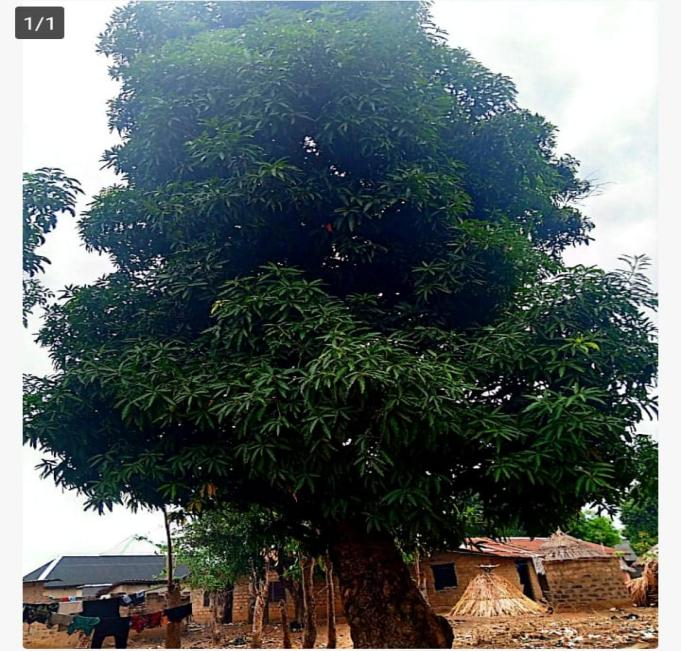
\includegraphics[width=3.09375in,height=2.95833in]{figures/media/image28.jpeg}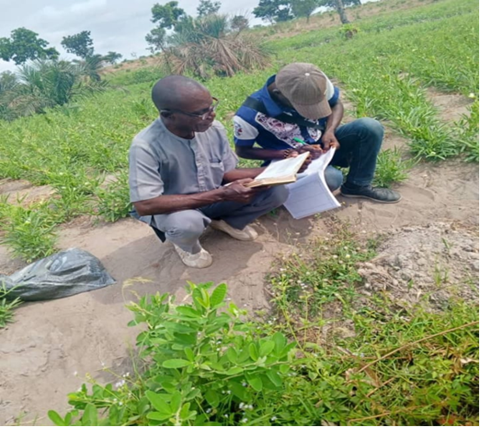
\includegraphics[width=3.2in,height=2.84722in]{figures/media/image29.png}\textbf{Field Work on Plants Species Diversity Data Collection}

Appendix 4

\includegraphics{figures/media/image30.emf}

Appendix 5

\includegraphics{figures/media/image31.emf}

Appendix 6

\includegraphics{figures/media/image32.emf}

Appendix 7

\includegraphics{figures/media/image33.emf}

Appendix 8

\includegraphics{figures/media/image34.emf}

Appendix 9

\includegraphics{figures/media/image35.emf}

Appendix 10

\begin{longtable}[]{@{}
  >{\raggedright\arraybackslash}p{(\columnwidth - 34\tabcolsep) * \real{0.0716}}
  >{\raggedright\arraybackslash}p{(\columnwidth - 34\tabcolsep) * \real{0.0733}}
  >{\raggedright\arraybackslash}p{(\columnwidth - 34\tabcolsep) * \real{0.0531}}
  >{\raggedright\arraybackslash}p{(\columnwidth - 34\tabcolsep) * \real{0.0524}}
  >{\raggedright\arraybackslash}p{(\columnwidth - 34\tabcolsep) * \real{0.0528}}
  >{\raggedright\arraybackslash}p{(\columnwidth - 34\tabcolsep) * \real{0.0537}}
  >{\raggedright\arraybackslash}p{(\columnwidth - 34\tabcolsep) * \real{0.0557}}
  >{\raggedright\arraybackslash}p{(\columnwidth - 34\tabcolsep) * \real{0.0546}}
  >{\raggedright\arraybackslash}p{(\columnwidth - 34\tabcolsep) * \real{0.0520}}
  >{\raggedright\arraybackslash}p{(\columnwidth - 34\tabcolsep) * \real{0.0520}}
  >{\raggedright\arraybackslash}p{(\columnwidth - 34\tabcolsep) * \real{0.0537}}
  >{\raggedright\arraybackslash}p{(\columnwidth - 34\tabcolsep) * \real{0.0549}}
  >{\raggedright\arraybackslash}p{(\columnwidth - 34\tabcolsep) * \real{0.0557}}
  >{\raggedright\arraybackslash}p{(\columnwidth - 34\tabcolsep) * \real{0.0540}}
  >{\raggedright\arraybackslash}p{(\columnwidth - 34\tabcolsep) * \real{0.0526}}
  >{\raggedright\arraybackslash}p{(\columnwidth - 34\tabcolsep) * \real{0.0540}}
  >{\raggedright\arraybackslash}p{(\columnwidth - 34\tabcolsep) * \real{0.0520}}
  >{\raggedright\arraybackslash}p{(\columnwidth - 34\tabcolsep) * \real{0.0520}}@{}}
\toprule\noalign{}
\endhead
\bottomrule\noalign{}
\endlastfoot
\multicolumn{18}{@{}>{\raggedright\arraybackslash}p{(\columnwidth - 34\tabcolsep) * \real{1.0000} + 34\tabcolsep}@{}}{%
\begin{minipage}[t]{\linewidth}\raggedright

NATIONAL POPULATION COMMISSION

ABUJA, NIGERIA

\end{minipage}} \\
\multicolumn{18}{@{}>{\raggedright\arraybackslash}p{(\columnwidth - 34\tabcolsep) * \real{1.0000} + 34\tabcolsep}@{}}{%
\begin{minipage}[t]{\linewidth}\raggedright

NATIONAL FIGURE FROM 2006 TO 2022

\end{minipage}} \\
\begin{minipage}[t]{\linewidth}\raggedright

STATE

\end{minipage} & \begin{minipage}[t]{\linewidth}\raggedright

2006

\end{minipage} & 2007 & 2008 & 2009 & 2010 & 2011 & 2012 & 2013 & 2014 & 2015 & 2016 & 2017 & 2018 & 2019 & 2020 & 2021 & 2022 \\
\begin{minipage}[t]{\linewidth}\raggedright

ABIA

\end{minipage} & 2,845,380 & 2,905,287 & 2,967,671 & 3,031,880 & 3,098,063 & 3,166,037 & 3,235,596 & 3,306,579 & 3,383,573 & 3,466,125 & 3,553,752 & 3,646,214 & 3,743,568 & 3,841,943 & 3,941,279 & 4,041,608 & 4,143,093 \\
\begin{minipage}[t]{\linewidth}\raggedright

ADAMAWA

\end{minipage} & 3,178,950 & 3,272,473 & 3,369,841 & 3,468,075 & 3,567,119 & 3,666,513 & 3,765,959 & 3,865,082 & 3,968,062 & 4,074,913 & 4,185,266 & 4,299,284 & 4,417,584 & 4,536,948 & 4,657,314 & 4,778,877 & 4,902,055 \\
\begin{minipage}[t]{\linewidth}\raggedright

AKWA IBOM

\end{minipage} & 3,902,051 & 3,963,247 & 4,027,113 & 4,092,733 & 4,159,871 & 4,228,237 & 4,297,421 & 4,367,206 & 4,437,200 & 4,507,044 & 4,576,294 & 4,644,867 & 4,712,967 & 4,780,581 & 4,847,542 & 4,913,809 & 4,979,418 \\
\begin{minipage}[t]{\linewidth}\raggedright

ANAMBRA

\end{minipage} & 4,177,828 & 4,286,534 & 4,397,524 & 4,505,444 & 4,610,707 & 4,713,143 & 4,812,262 & 4,907,709 & 5,010,207 & 5,118,973 & 5,233,407 & 5,352,877 & 5,477,532 & 5,599,910 & 5,720,035 & 5,837,646 & 5,953,517 \\
\begin{minipage}[t]{\linewidth}\raggedright

BAUCHI

\end{minipage} & 4,653,066 & 4,847,876 & 5,047,406 & 5,252,679 & 5,464,244 & 5,682,270 & 5,907,203 & 6,139,446 & 6,371,216 & 6,603,199 & 6,835,118 & 7,067,129 & 7,300,050 & 7,540,663 & 7,788,504 & 8,043,978 & 8,308,783 \\
\begin{minipage}[t]{\linewidth}\raggedright

Bayelsa

\end{minipage} & 1,704,515 & 1,761,197 & 1,819,103 & 1,875,276 & 1,929,864 & 1,982,672 & 2,033,433 & 2,081,965 & 2,132,192 & 2,183,880 & 2,236,872 & 2,290,985 & 2,343,687 & 2,394,725 & 2,444,028 & 2,491,513 & 2,537,375 \\
\begin{minipage}[t]{\linewidth}\raggedright

BENUE

\end{minipage} & 4,253,641 & 4,365,768 & 4,483,938 & 4,602,120 & 4,720,509 & 4,839,060 & 4,957,574 & 5,076,012 & 5,195,024 & 5,314,166 & 5,432,973 & 5,551,238 & 5,669,555 & 5,787,706 & 5,905,747 & 6,023,643 & 6,141,284 \\
\begin{minipage}[t]{\linewidth}\raggedright

BORNO

\end{minipage} & 4,171,104 & 4,311,697 & 4,456,293 & 4,590,977 & 4,716,157 & 4,831,836 & 4,937,582 & 5,033,360 & 5,137,240 & 5,248,555 & 5,366,703 & 5,491,442 & 5,623,677 & 5,751,590 & 5,875,471 & 5,995,271 & 6,111,462 \\
\begin{minipage}[t]{\linewidth}\raggedright

CROSS RIVER

\end{minipage} & 2,892,988 & 2,987,619 & 3,085,111 & 3,185,687 & 3,289,317 & 3,395,946 & 3,505,493 & 3,617,904 & 3,725,751 & 3,828,099 & 3,924,082 & 4,013,047 & 4,094,739 & 4,175,020 & 4,253,698 & 4,330,767 & 4,406,204 \\
\begin{minipage}[t]{\linewidth}\raggedright

DELTA

\end{minipage} & 4,112,445 & 4,192,014 & 4,275,075 & 4,358,889 & 4,443,441 & 4,528,537 & 4,613,842 & 4,699,157 & 4,789,960 & 4,885,710 & 4,985,899 & 5,090,103 & 5,198,675 & 5,307,543 & 5,416,738 & 5,526,218 & 5,636,145 \\
\begin{minipage}[t]{\linewidth}\raggedright

EBONYI

\end{minipage} & 2,176,947 & 2,230,021 & 2,285,259 & 2,342,009 & 2,400,297 & 2,460,053 & 2,521,131 & 2,583,471 & 2,648,349 & 2,715,675 & 2,785,306 & 2,857,120 & 2,931,444 & 2,931,444 & 3,084,214 & 3,162,510 & 3,242,518 \\
\begin{minipage}[t]{\linewidth}\raggedright

EDO

\end{minipage} & 3,233,366 & 3,322,668 & 3,414,774 & 3,505,653 & 3,595,335 & 3,683,611 & 3,770,141 & 3,854,642 & 3,944,847 & 4,040,178 & 4,140,181 & 4,244,511 & 4,353,500 & 4,461,137 & 4,567,512 & 4,672,707 & 4,777,042 \\
\begin{minipage}[t]{\linewidth}\raggedright

EKITI

\end{minipage} & 2,398,957 & 2,464,735 & 2,532,953 & 2,601,870 & 2,671,288 & 2,740,939 & 2,810,358 & 2,879,180 & 2,951,454 & 2,951,454 & 3,104,755 & 3,185,220 & 3,268,175 & 3,350,401 & 3,431,742 & 3,512,293 & 3,592,163 \\
\begin{minipage}[t]{\linewidth}\raggedright

ENUGU

\end{minipage} & 3,267,837 & 3,332,691 & 3,400,471 & 3,473,924 & 3,553,158 & 3,637,979 & 3,728,114 & 3,823,387 & 3,917,615 & 4,010,294 & 4,100,649 & 4,188,334 & 4,273,288 & 4,396,098 & 4,505,928 & 4,603,802 & 4,690,053 \\
\begin{minipage}[t]{\linewidth}\raggedright

GOMBE

\end{minipage} & 3,267,837 & 2,448,350 & 2,534,438 & 2,623,049 & 2,714,145 & 2,807,884 & 2,904,216 & 3,003,456 & 3,103,782 & 3,205,287 & 3,307,801 & 3,411,323 & 3,516,217 & 3,623,462 & 3,733,100 & 3,845,132 & 3,960,122 \\
\begin{minipage}[t]{\linewidth}\raggedright

IMO

\end{minipage} & 3,927,563 & 4,011,289 & 4,097,660 & 4,187,079 & 4,279,489 & 4,374,817 & 4,472,606 & 4,572,581 & 4,673,183 & 4,773,738 & 4,873,654 & 4,972,386 & 5,070,149 & 5,167,722 & 5,265,082 & 5,362,138 & 5,459,337 \\
\begin{minipage}[t]{\linewidth}\raggedright

JIGAWA

\end{minipage} & 4,361,002 & 4,505,748 & 4,655,575 & 4,814,643 & 4,983,139 & 5,161,158 & 5,349,168 & 5,547,687 & 5,747,033 & 5,947,966 & 6,150,337 & 6,354,507 & 6,561,451 & 6,779,080 & 7,007,317 & 7,246,906 & 7,499,059 \\
\begin{minipage}[t]{\linewidth}\raggedright

KADUNA

\end{minipage} & 6,113,503 & 6,279,678 & 6,454,239 & 6,620,107 & 6,776,631 & 6,922,330 & 7,055,966 & 7,176,135 & 7,320,414 & 7,487,845 & 7,678,078 & 7,891,256 & 8,105,251 & 8,324,285 & 8,549,066 & 8,779,665 & 9,032,181 \\
\begin{minipage}[t]{\linewidth}\raggedright

KANO

\end{minipage} & 9,401,288 & 9,774,482 & 10,157,318 & 10,531,655 & 10,898,900 & 11,259,361 & 11,612,318 & 11,958,431 & 12,315,760 & 12,683,756 & 13,061,860 & 13,450,530 & 13,852,238 & 14,253,549 & 14,655,311 & 15,057,715 & 15,462,177 \\
\begin{minipage}[t]{\linewidth}\raggedright

KATSINA

\end{minipage} & 5,801,584 & 6,023,815 & 6,252,815 & 6,488,761 & 6,732,529 & 6,984,729 & 7,245,828 & 7,516,462 & 7,793,967 & 7,793,967 & 8,369,926 & 8,668,899 & 8,977,242 & 9,300,382 & 9,639,059 & 9,994,288 & 10,368,483 \\
\begin{minipage}[t]{\linewidth}\raggedright

KEBBI

\end{minipage} & 3,256,541 & 3,360,340 & 3,468,467 & 3,582,255 & 3,701,785 & 3,826,955 & 3,957,728 & 4,094,168 & 4,234,095 & 4,377,770 & 4,525,293 & 4,677,379 & 4,834,886 & 5,001,610 & 5,178,123 & 5,365,330 & 5,563,907 \\
\begin{minipage}[t]{\linewidth}\raggedright

KOGI

\end{minipage} & 3,314,043 & 3,352,369 & 3,396,391 & 3,444,522 & 3,496,074 & 3,550,841 & 3,608,382 & 3,668,755 & 3,734,782 & 3,806,551 & 3,884,218 & 3,967,919 & 4,058,704 & 4,153,734 & 4,253,371 & 4,357,794 & 4,466,801 \\
\begin{minipage}[t]{\linewidth}\raggedright

KWARA

\end{minipage} & 2,365,353 & 2,415,629 & 2,468,744 & 2,525,690 & 2,586,148 & 2,650,004 & 2,716,873 & 2,786,756 & 2,858,762 & 2,933,031 & 3,009,755 & 3,089,231 & 3,172,216 & 3,259,613 & 3,351,720 & 3,448,777 & 3,551,023 \\
\begin{minipage}[t]{\linewidth}\raggedright

LAGOS

\end{minipage} & 9,113,605 & 9,383,057 & 9,660,057 & 9,948,305 & 10,246,131 & 10,551,625 & 10,862,618 & 11,177,409 & 11,477,699 & 11,763,161 & 12,033,445 & 12,288,839 & 12,531,530 & 12,772,884 & 13,012,971 & 13,252,387 & 13,491,804 \\
\begin{minipage}[t]{\linewidth}\raggedright

NASSARAWA

\end{minipage} & 1,869,377 & 1,908,465 & 1,950,560 & 1,996,715 & 2,046,759 & 2,100,608 & 2,158,187 & 2,219,522 & 2,282,745 & 2,282,745 & 2,347,955 & 2,484,482 & 2,556,350 & 2,632,239 & 2,712,349 & 2,796,947 & 2,886,022 \\
\begin{minipage}[t]{\linewidth}\raggedright

NIGER

\end{minipage} & 3,954,772 & 4,122,414 & 4,295,946 & 4,468,171 & 4,639,280 & 4,808,915 & 4,976,757 & 5,142,705 & 5,313,102 & 5,487,607 & 5,665,810 & 5,847,657 & 6,033,997 & 6,220,617 & 6,407,568 & 6,594,892 & 6,783,325 \\
\begin{minipage}[t]{\linewidth}\raggedright

OGUN

\end{minipage} & 3,751,140 & 3,912,666 & 4,078,465 & 4,249,256 & 4,424,849 & 4,605,110 & 4,789,518 & 4,977,824 & 5,158,612 & 5,331,389 & 5,495,738 & 5,651,466 & 5,798,744 & 5,945,275 & 6,090,740 & 6,235,389 & 6,379,532 \\
\begin{minipage}[t]{\linewidth}\raggedright

ONDO

\end{minipage} & 3,460,877 & 3,561,438 & 3,665,577 & 3,774,531 & 3,888,324 & 4,007,005 & 4,130,312 & 4,258,213 & 4,384,163 & 4,507,463 & 4,627,488 & 4,743,667 & 4,856,143 & 4,969,707 & 5,084,330 & 5,199,832 & 5,316,603 \\
\begin{minipage}[t]{\linewidth}\raggedright

OSUN

\end{minipage} & 3,416,959 & 3,469,426 & 3,524,558 & 3,582,296 & 3,642,607 & 3,705,505 & 3,770,635 & 3,837,823 & 3,905,483 & 3,973,037 & 4,040,045 & 4,106,177 & 4,171,661 & 4,237,396 & 4,303,366 & 4,369,473 & 4,435,803 \\
\begin{minipage}[t]{\linewidth}\raggedright

OYO

\end{minipage} & 5,580,894 & 5,724,321 & 5,870,883 & 6,017,535 & 6,164,227 & 6,310,726 & 6,456,569 & 6,601,542 & 6,749,107 & 6,898,796 & 7,050,013 & 7,202,908 & 7,358,018 & 7,512,855 & 7,667,318 & 7,821,434 & 7,976,081 \\
\begin{minipage}[t]{\linewidth}\raggedright

PLATEAU

\end{minipage} & 3,206,531 & 3,281,149 & 3,360,760 & 3,444,191 & 3,531,259 & 3,714,915 & 3,811,162 & 3,907,945 & 3,907,945 & 4,005,406 & 4,103,256 & 4,201,252 & 4,300,001 & 4,400,974 & 4,504,272 & 4,609,669 & 4,717,305 \\
\begin{minipage}[t]{\linewidth}\raggedright

RIVERS

\end{minipage} & 5,198,716 & 5,328,162 & 5,462,088 & 5,598,197 & 5,736,180 & 5,875,350 & 6,014,630 & 6,153,094 & 6,294,653 & 6,439,012 & 6,585,693 & 6,734,279 & 6,885,307 & 7,034,973 & 7,183,473 & 7,330,764 & 7,476,805 \\
\begin{minipage}[t]{\linewidth}\raggedright

SOKOTO

\end{minipage} & 3,702,676 & 3,866,216 & 4,033,171 & 4,199,311 & 4,364,153 & 4,527,047 & 4,687,262 & 4,844,245 & 5,004,659 & 5,168,672 & 5,336,484 & 5,508,650 & 5,686,341 & 5,863,187 & 6,039,289 & 6,214,881 & 6,391,047 \\
\begin{minipage}[t]{\linewidth}\raggedright

TARABA

\end{minipage} & 2,294,800 & 2,360,112 & 2,428,624 & 2,500,644 & 2,576,092 & 2,654,897 & 2,736,961 & 2,822,424 & 2,907,564 & 2,992,417 & 3,076,898 & 3,160,982 & 3,245,094 & 3,331,885 & 3,421,510 & 3,514,117 & 3,609,843 \\
\begin{minipage}[t]{\linewidth}\raggedright

YOBE

\end{minipage} & 2,321,339 & 2,405,685 & 2,492,327 & 2,577,228 & 2,660,844 & 2,824,673 & 2,904,997 & 2,986,104 & 3,067,883 & 3,150,002 & 3,232,244 & 3,315,082 & 3,398,177 & 3,481,567 & 3,565,258 & 3,565,258 & 3,649,607 \\
\begin{minipage}[t]{\linewidth}\raggedright

ZAMFARA

\end{minipage} & 1,406,239 & 3,407,567 & 3,539,989 & 3,681,136 & 3,831,298 & 3,991,000 & 4,160,798 & 4,341,427 & 4,516,743 & 4,686,636 & 4,850,510 & 5,008,075 & 5,159,678 & 5,317,793 & 5,482,423 & 5,654,021 & 5,833,494 \\
\begin{minipage}[t]{\linewidth}\raggedright

FCT ABUJA

\end{minipage} & 1,406,239 & 1,489,957 & 1,576,504 & 1,665,938 & 1,758,208 & 1,853,377 & 1,951,425 & 2,052,494 & 2,155,943 & 2,261,377 & 2,368,558 & 2,477,433 & 2,588,192 & 2,702,443 & 2,820,261 & 2,941,873 & 3,067,457 \\
\begin{minipage}[t]{\linewidth}\raggedright

TOTAL

\end{minipage} & 140,431,790 & 144,636,162 & 148,987,688 & 153,408,431 & 157,898,421 & 162,625,665 & 167,231,025 & 171,882,302 & 176,520,769 & 180,905,896 & 186,136,316 & 191,136,750 & 196,126,028 & 201,142,941 & 206,367,029 & 211,493,324 & 216,798,930 \\
\end{longtable}

Appendix 11 data collection acknowledgement letters

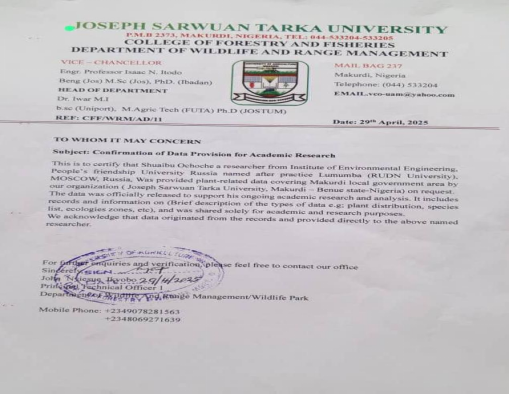
\includegraphics[width=6.41667in,height=8.19792in]{figures/media/image36.png}


\includegraphics[width=6.45833in,height=7.5in]{figures/media/image37.png}
